\section{Preliminary Work}

All code is available from \url{https://github.com/kewiechecki/DeePWAK}. 

\subsection{Overview}
\subsubsection{Clusters obtained by $KE$ decomposition accurately predict the behavior of an outer model}
I trained a toy outer model with a 3 neuron information bottleneck.
I used two encoder methods to split the bottleneck activations into features.
A na\"ive SAE successfully split the bottleneck into sparse features.
Adding 
\subsubsection{Multihead $KE$ decomposition splits major and minor features}

\subsubsection{Features appear consistently bisemantic}

\subsection{Proposed Followup Experiments}
look for clusters in an autoencoder rather than a classifier
What do the cluster centroids look like at different points in training?
What do feature ablations do in SAE vs. PSAE?

I expect the encoder-decoder methods to converge over enough training time.
I expect clusters to become more defined as loss decreases.
I'm hoping to see grokking.
I expect feature ablations to produce more interpretable results in PSAE than SAE.

***I expect the outer classifier and outer autoencoder to have similar representations in the bottleneck.***

write decoder
rewrite training to save checkpoints
write centroid calculation function
write decoder viz plots
write ablation tests
clean up data viz code to put on github
clean up repo documentation
add figure for loss
remove outline scale from dot plot
describe hypergeometric test



\subsubsection{How do representative cluster members develop during training?}

\subsubsection{Can we observe grokking?}

\subsubsection{Why bisemanticity?}

\subsubsection{How can these methods be applied to an LLM?}
\subsection{DeePWAK}

Our basic unit performing clustering is the \DeePWAK head.
It is a deep learning architecture consisting of an encoder, partitioner, and decoder subnetworks.
%Details are in Appendix \ref{app:DeePWAK}.


\begin{figure}
     \begin{subfigure}[b]{0.5\textwidth}
        \begin{tikzpicture}[
    node distance = 5mm and 5mm,
    punkt/.style = {rectangle, draw},
    pil/.style = {black, -stealth},
    font=\small
    ]

  %\node[punkt] (preprocessing) {preprocessing} ;
  \node[] (X) {$X^{m \times n}$} ;
  \node[punkt] (encoder) [below=of X] {$\encoder^{m \to d}$} ;
  \node[] (E) [below=of encoder] {$E^{d \times n}$} ;
  \node[punkt] (Etranspose) [below=of E] {\transpose} ;

  \node[punkt] (partitioner) [left=of encoder] {$\partitioner^{m \to k}$} ;
  \node[punkt] (softmax) [below=of partitioner] {\softmax} ;

  \node[] (K) [below=of softmax] {$K^{k \times n}$} ;
  %\node[punkt] (Ktranspose) [left=of K] {\transpose} ;
  %\node[punkt] (KK) [below=of Ktranspose] {\matmul} ;
  %\node[] (P) [below=of KK] {$P^{n \times n}$} ;
  \node[punkt] (wak) [below=of K] {\PWAK} ;
  \node[punkt] (GE) [below=of Etranspose] {\matmul} ;
  \node[] (Ehat) [below=of GE] {$\hat{E}^{d \times n}$} ;

  \node[punkt] (decoder) [left=of Ehat] {$\decoder^{d \to m}$} ;
  \node[] (Xhat) [left=of decoder] {$\hat{X}^{m \times n}$} ;

  \draw[pil] %(preprocessing) edge (X)
  (X) edge (encoder)
  (encoder) edge (E)
  (E) edge (Etranspose)
  (Etranspose) edge (GE)
  
  (X) edge (partitioner)
  (partitioner) edge (softmax)
  (softmax) edge (K)
  (K) edge (wak)
  %(Ktranspose) edge (KK)
  %(K) edge (KK)
  %(KK) edge (P)
  %(P) edge (wak)
  (wak) edge (GE)
  (GE) edge (Ehat)

  (Ehat) edge (decoder)
  (decoder) edge (Xhat);
\end{tikzpicture}


         \caption{}
         \label{fig:}
     \end{subfigure}
     \hfill
     \begin{subfigure}[b]{\textwidth}
        \begin{tikzpicture}[
    node distance = 5mm and 5mm,
    punkt/.style = {rectangle, draw},
    pil/.style = {black, -stealth},
    font=\small
    ]

  %\node[punkt] (preprocessing) {preprocessing} ;
  \node[] (X) {$X$} ;

  \node[punkt] (h3) [right=of X] {$\mathDeePWAK$} ;
  \node[punkt] (h2) [above=of h3] {$\mathDeePWAK$} ;
  \node[punkt] (h1) [above=of h2] {$\mathDeePWAK$} ;
  \node[punkt] (h4) [below=of h3] {$\mathDeePWAK$} ;
  \node[punkt] (h5) [below=of h4] {$\mathDeePWAK$} ;

  %\node[] (Xhat1) [below=of h1] {$\hat{X}_1$} ;
  %\node[] (Xhat2) [below=of h2] {$\hat{X}_2$} ;
  %\node[] (Xhat3) [below=of h3] {$\hat{X}_3$} ;
  %\node[] (Xhat4) [below=of h4] {$\hat{X}_4$} ;
  %\node[] (Xhat5) [below=of h5] {$\hat{X}_5$} ;

  %\node[punkt] (sum) [right=of h3] {$\sum$} ;
  \node[] (concat) [right=of h3] {$\oplus$} ;
  \node[punkt] (linear) [right=of concat] {$\linear^{5 \times m \to m}$} ;
  \node[] (Xhat) [right=of linear] {$\hat{X}$} ;
  %\node[punkt] (loss) [below=of h5] {MSE} ;
  %\node[] (grad) [right=of loss] {$\nabla$} ;
  %\node[punkt] (update) [right=of grad] {$\mathrm{update!}(\theta,\pi,\phi)$} ;
  
  \draw[pil] %(preprocessing) edge (X)

  (X) edge[bend left=30] (h1)
  (X) edge[bend left=30] (h2)
  (X) edge (h3)
  (X) edge[bend right=30] (h4)
  (X) edge[bend right=30] (h5)

  (h1) edge[bend left=30] (concat)
  (h2) edge[bend left=30] (concat)
  (h3) edge (concat)
  (h4) edge[bend right=30] (concat)
  (h5) edge[bend right=30] (concat)

  (concat) edge (linear)
  (linear) edge (Xhat) ;
  %(sum) edge[bend left=15] (Xhat) ;
  %(Xhat) edge[bend left=15] (loss) 
  %(X) edge[bend right=30] (loss)
  %(loss) edge (grad)
  %(grad) edge (update);
\end{tikzpicture}

  

         \caption{}
         \label{fig:}
     \end{subfigure}

     \caption{
       (a) Architecture of one DeePWAK head.
       (b) Architecture of one DeePWAK block with $h=5$.}
     \label{fig:deepwak}
\end{figure}
  
\subsection{Ensemble $\mathDeePWAK$}

\DeePWAK can be used for ensemble clustering by training multiple heads in parallel and linearly combining the results.
We refer to this as a \DeePWAKBlock.
An intuitive interpretation is that each head learns to cluster a different ``slice'' of the data.

\subsection{PSAE}
A modified version of \DeePWAK is to insert a partitioner between the encoding and decoding step of a SAE.

\subsection{A toy model of feature splitting}
I trained a MNIST classifier with a 3 neuron bottleneck.
I hypothesized that since the model had more labels than neurons in the bottleneck, features would be represented in superposition.
I refer to this as the ``outer model''.
I train three ``inner models'' which try to predict the outer model's predictions from the bottleneck activations.
These are a na\"ive SAE, a PSAE, and a DeePWAK.
All models have an embedding size of 27.
The PSAE is identical to the SAE except for containing a partitioner submodel.
Both the PSAE and DeePWAK inner models have identical partitioner subnetworks with a maximum $k$ of 12.
They only differ in their encoders and (in the case of DeePWAK) decoders.

\subsubsection{How to read the figures}
Heatmaps are ubiquitous in bioinformatics for visualizing very large data sets.
In Fig. \ref{fig:E_MNIST} and \ref{fig:K_MNIST}, rows are samples and columns are activations.
Samples are split either by training label (Fig. \ref{fig:E_MNIST}) or predicted label (Fig. \ref{fig:K_MNIST}.
Activations are split by model.
For Fig. \ref{fig:E_MNIST}, these are the encoder activations.
\textsf{bottleneck} gives the bottleneck activations for the outer model.
\textsf{SAE} gives 


\begin{figure}
  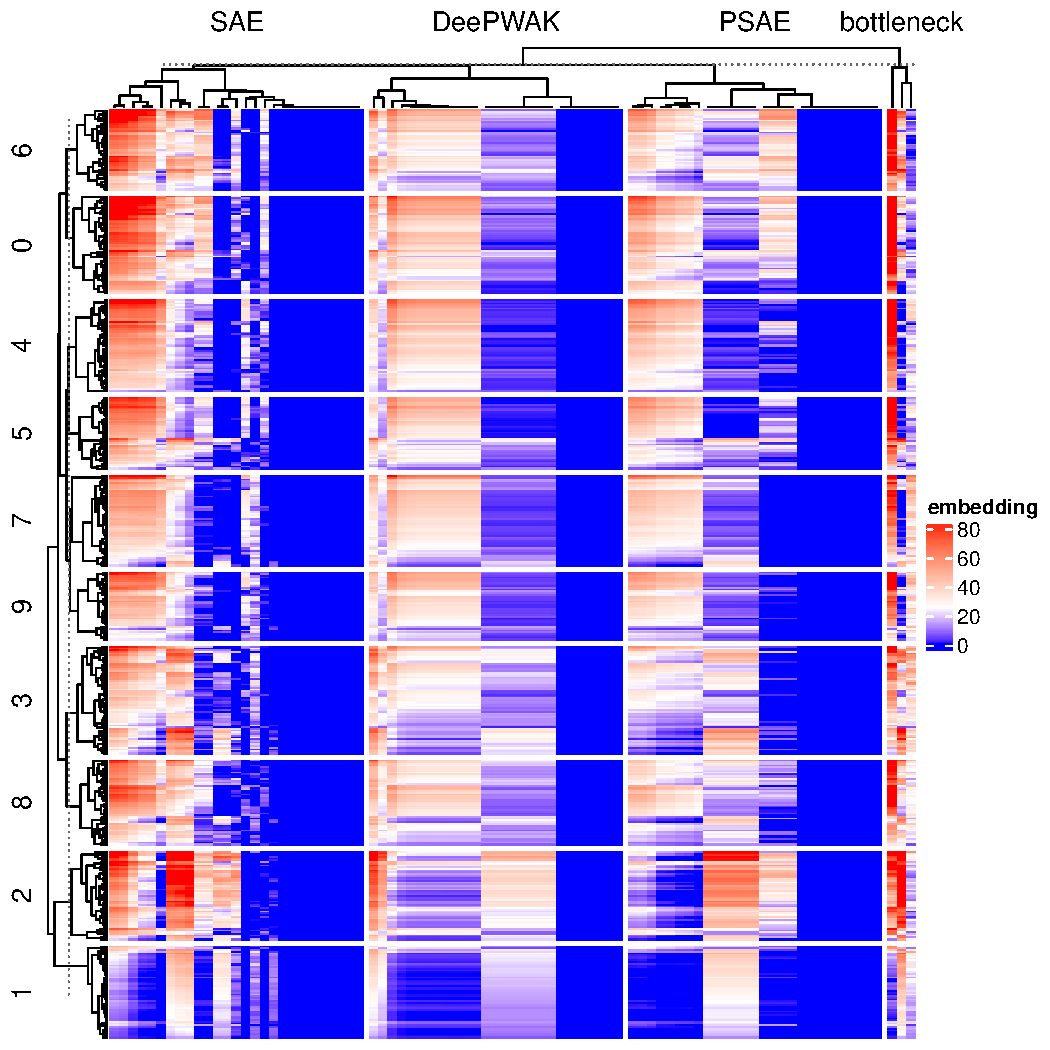
\includegraphics[width=\textwidth]{E_labels.pdf}
  \caption{Feature splitting of bottleneck activations by different methods.
    There is a clear progression of sparcity from a na\"ive SAE, PSAE, and DeePWAK.
    Rows are split by training set label.
    Interestingly, adding a partitioner submodel seems to result in the same feature being copied by multiple embeddings.}
    \label{fig:E_MNIST}
\end{figure}

\begin{figure}
  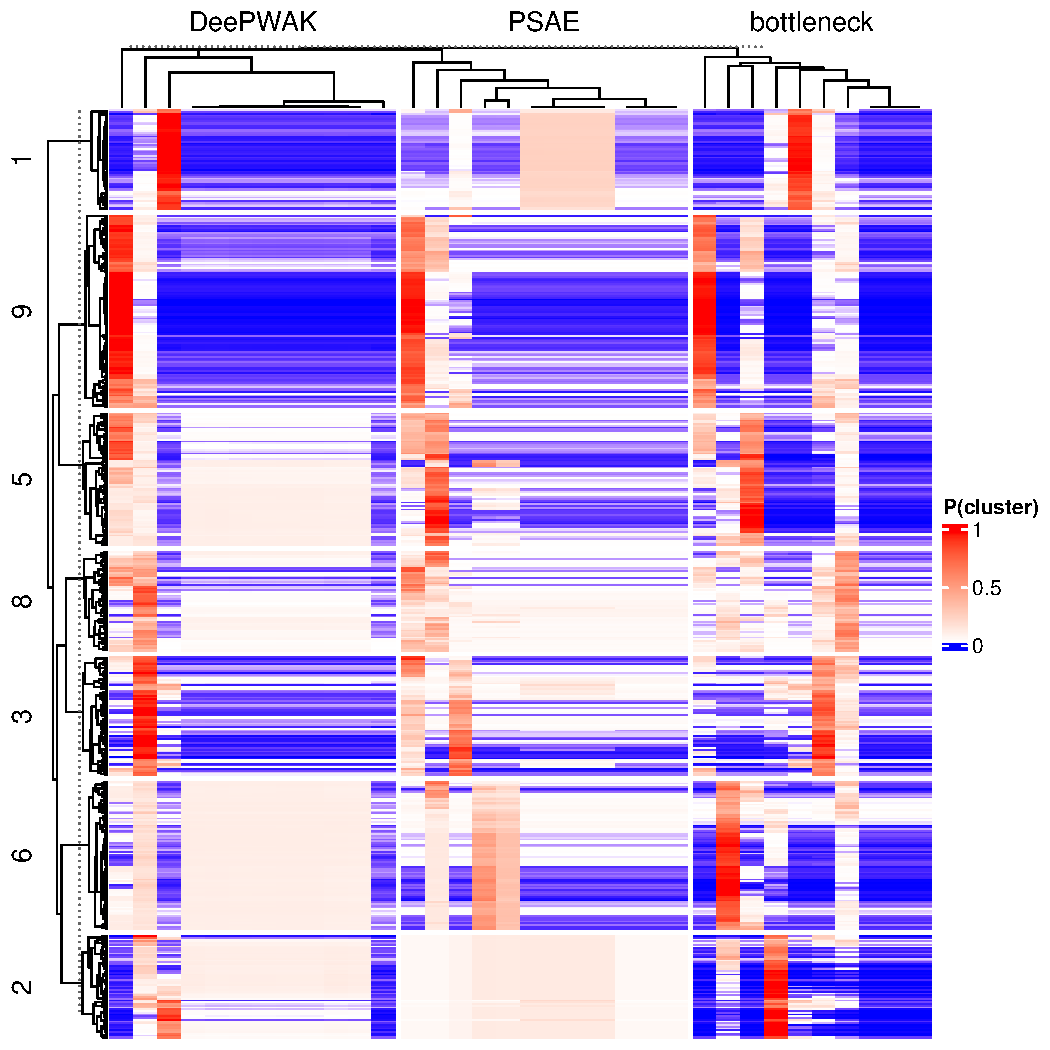
\includegraphics[width=\textwidth]{K_predicted.pdf}
    \caption{Both DeePWAK and PSEA learn sparse clusters. Rows are split by predicted label.}
    \label{fig:K_MNIST}
\end{figure}

\begin{figure}
  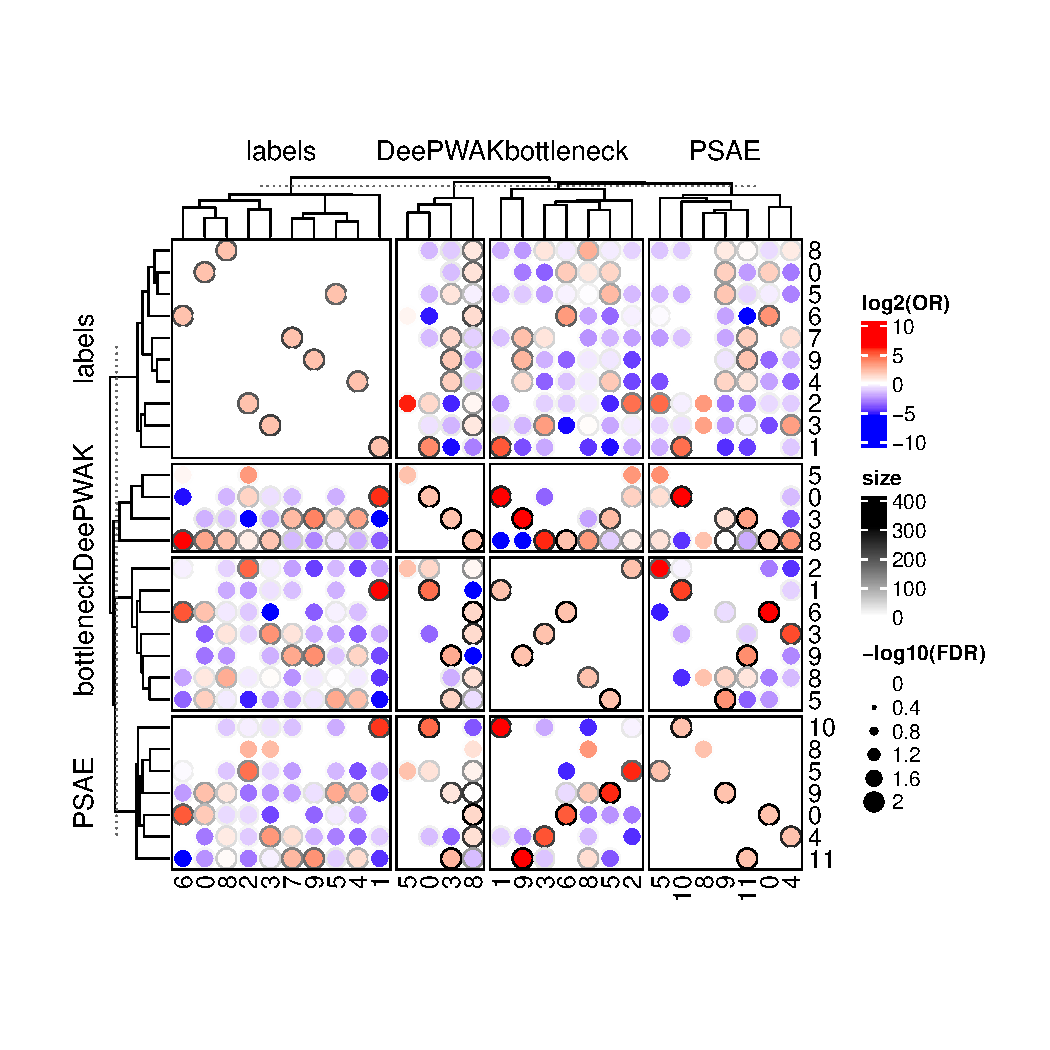
\includegraphics[width=\textwidth]{enrichment.pdf}
    \caption{Hypergeometric test for enrichment of [rows] in [columns].}
    \label{fig:hyperMNIST}
\end{figure}

Even trained without a sparcity correction, \DeePWAK finds a more sparse representation than the SAE or PSAE (Fig. \ref{fig:E_MNIST}, \ref{fig:K_MNIST}.

Both DeePWAK and PSAE seem to capture latent features from the bottleneck (Fig. \ref{fig:hyperMNIST}.
Strikingly, PSAE better predicts the model output than the model predicts the training labels.
DeePWAK, on the other hand, appears to identify higher level features used by the model for classification.
It reveals the model apparently grouping rounded (0,3,6,8) and pointed (4,5,7,9) digits. 
Even more curiously, these features appear \textit{bisemantic}.
Looking at \textsf{DeePWAK 0}, this cluster appears to regard 6 as ``opposite'' of 1.
If we look back at Fig. \ref{fig:K_MNIST}, we can see the partitioner is much less confident classifying 6s than other digits.
It's possible the model is using an internal logic of ``I don't know what this is but it's definitely not a 1''.

\subsection{Ensemble $\mathDeePWAK$ separates major and minor features}

\begin{figure}
  %\begin{subfigure}[b]{0.5\textwidth}
  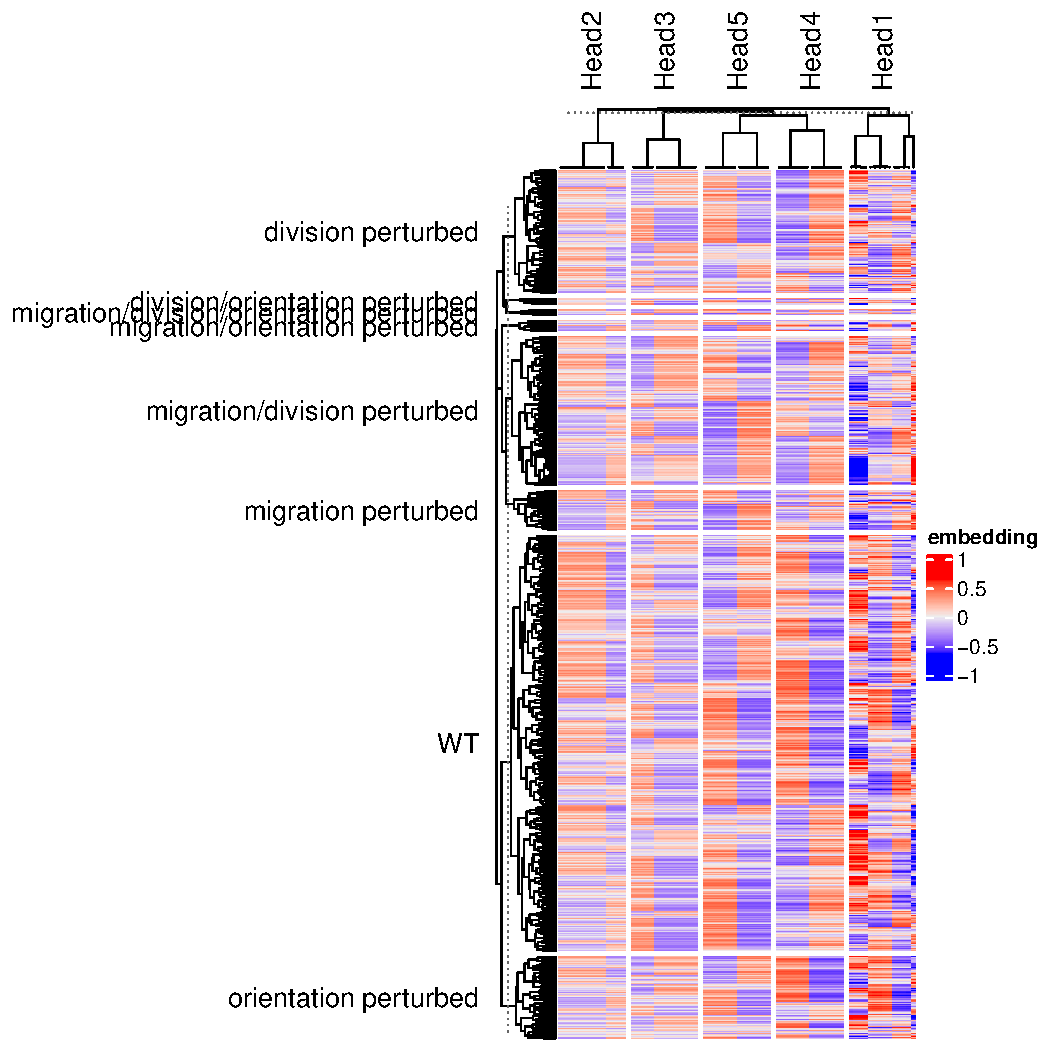
\includegraphics[width=\textwidth]{embeddings.pdf}
    \caption{Ensemble DeePWAK learns sparse embedding values. Interestingly, most heads learn two directly opposing features.}
    \label{fig:blockE}
\end{figure}

    
\begin{figure}
  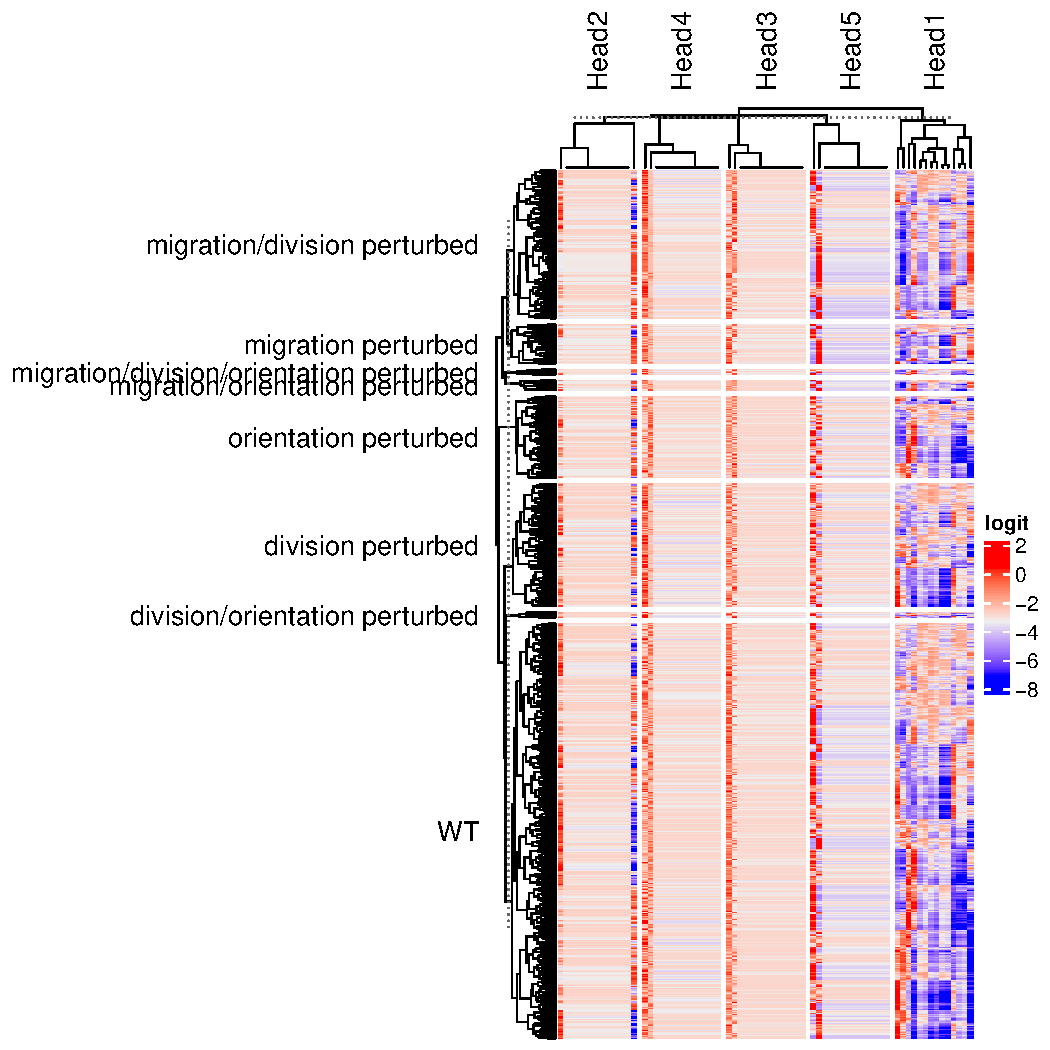
\includegraphics[width=\textwidth]{logits.pdf}
  \caption{For most heads, two clusters dominate.}
  \label{fig:blockK}
\end{figure}

\begin{figure}
  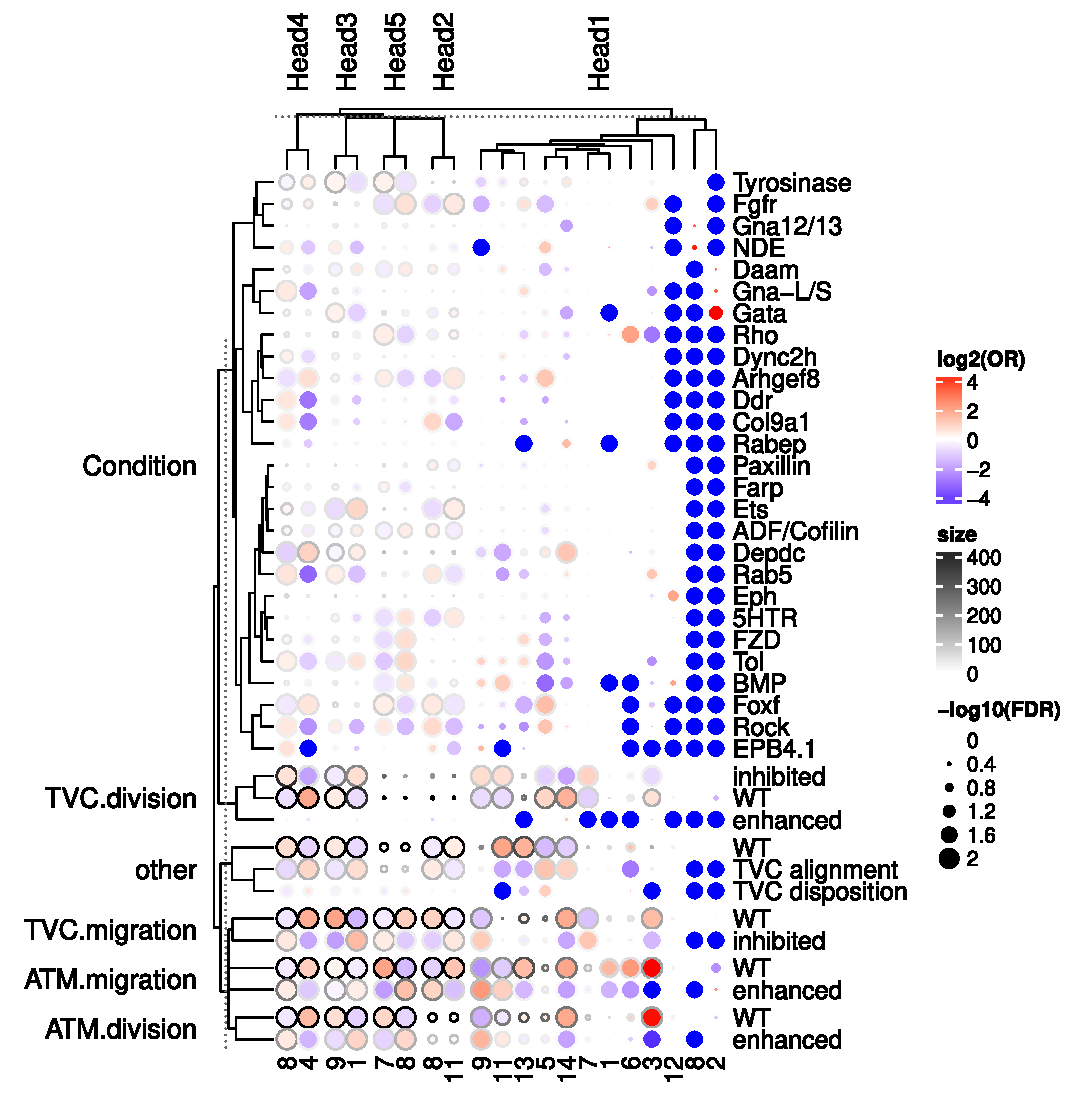
\includegraphics[width=\textwidth]{phenotype.pdf}
  \caption{Hypergeometric test for enrichment of phenotype and treatment condition for each cluster in each head. Dot color indicates overrepresentation of each category in a cluster compared to a uniform prior. Dot size indicates statistical significance of the difference. Dot outline shade indicates number of embryos represented by a dot. \textsf{Head1} appears ``polysemantic''. The others appear to distinguish single phenotypic categories.}
  \label{fig:hyper}
\end{figure}

Multihead \DeePWAK learns remarkably sparse features (Fig. \ref{fig:blockE}) and clusters (Fig. \ref{fig:blockK}). 
Even more remarkably, all but one head appear bisemantic.
This is suggestive that the model may in fact be learning a tree structure to split the data along major features. These major features effectively split experimenter-labeled phenotypes (Fig. \ref{fig:hyper}). 

All of the more nuanced discrimination happens in \textsf{Head1}.
It splits the data into almost but not quite the maximum number of clusters, indicating our choice of $k$ is close to the latent concept space for (this projection of) the data.
Fascinatingly, the embeddings are even sparcer.

\section{Plan}

\subsection{Can we split DeePWAK features?}
\DeePWAK seems to capture more general features than PSAE.
It would be very useful if we could express high level features as compositions of lowe level features.

\subsection{Why bisemanticity?}
This is the biggest question I have. It shows up prominently in two very different data sets using different analyses.
It suggests that monosemantic features may not be the most ``natural'' way to represent data.
The previous analogy to PCA may be informative.
If there is no privileged basis in feature space, it seems likely that features attempt to capture the vectors of highest variance.

\subsection{Experiments on GPT2}
Adapting DeePWAK to LLMs will present challenges.
In its current form it performs poorly when the number of latent clusters is much larger than the minibatch size.
A possible workaround is to add a dictionary of representative ``platonic forms'' that are appended to each minibatch.

\paragraph{Is a nonlinear decoder necessary?}

\paragraph{How decomposable are clusters?}

\paragraph{What makes a cluster ``interpretable''?}

\paragraph{Can we get a recurrent ontology?}
